\chapter{Kết quả thực nghiệm}
\ifpdf
\graphicspath{{Chapter4/Chapter4Figs/PNG/}{Chapter4/Chapter4Figs/PDF/}{Chapter4/Chapter4Figs/}}
\else
\graphicspath{{Chapter4/Chapter4Figs/EPS/}{Chapter4/Chapter4Figs/}}
\fi
\begin{quote}
	\textit{Trong chương này sẽ trình bày chi tiết về cấu trúc mô hình mà chúng em đã thiết lập. Đồng thời đề cập đến những phương pháp để đánh giá mô hình học và những kết quả thực nghiệm đã nhận được. Qua đó so sánh với các phương pháp đã đề xuất trước đây để thấy được tính hiệu quả của mô hình này.}
\end{quote}
 
\section{Giới thiệu Arcade Learning Environment}
Arcade Learning Environment (ALE) là một framework được thiết kế giúp dễ dàng trong việc phát triển những hệ thống có thể tự động chơi bất kỳ những game trên hệ máy Atari 2600.
\subsection{Hệ máy Atari 2600}
\ref{fig:AtariConsole} là hệ máy chơi game Atari 2600 tại gia đình được phát triển và sử dụng phổ biến vào những năm 1970.
Hơn 500 game đã được phát triển cho hệ máy này; một số game vẫn tiếp tục được phát triển cho tới ngày nay. Độ phân giải của những game này là $210 \times 160$. Mặc dù vậy nhiều game được phát triển cho hệ máy này, nhưng cấu hình phần cứng của chúng khá đơn giản bao gồm một CPU 1.19 Mhz, một bộ nhớ ROM 2-4KB để lưu giữ code của game, và dung lượng RAM của máy cũng chỉ là 128 bytes. Đồ họa của các game được cố định ở độ phân giải $160 x 210$, với ảnh màu RGB. Người chơi tương tác với game qua một thiết bị được gọi là joystick, có thể thực hiện tối đa 18 hành động.

\subsection{Interface}
ALE được xây dựng trên nền Stella, nó giả lập máy hệ máy Atari 2600. Qua đó cho phép người dùng tương tác với Atari 2600 bằng cách tiếp nhận những di chuyển của joystick, gửi thông tin của game cho người dùng như hình ảnh, điểm số nhận được. ALE cũng cung cấp một \textit{lớp sử lý} để chuyển đổi những thông tin trong game theo chuẩn của bài toán học tăng cường như điểm số đạt được, kết thúc game chưa. Mặc định, lớp này biểu diễn mỗi trạng thái trong game bằng một mảng 7-bit pixels 2 chiều, và không gian hành động gồm 18 hành động tương ứng với các hành động có thể thực hiện trong joystick. Lớp sử lý cung cấp thông tin tập những hành động cụ thể có thể thực hiện trong một game. ALE có thể tạo ra 60 frame hình ảnh game trong một giây theo mặc định, và số frame ảnh nhiều nhất trong một giây nó có thể tạo ra 6000 frame. Điểm số nhận được tại từng thời điểm được định nghĩa theo từng game khác nhau. Một mẫu thực nghiệm có thể được tao ra từ frame đầu tiên của game cho đến khi game kết thúc, ngoài ra lớp sử lý cũng cho phép người người tạo mãu thực nghiệm với số lượng frame cố định.

ALE hơn nữa cũng cung cấp chức năng \textit{sao lưu} và \textit{khôi phục} trạng thái của game. Khi lệnh sao lưu được thực thi, ALE lưu lại tất cả các dữ liệu liên quan tại thời điểm đó trong game như nội dung RAM, registers. Ngược lại khi lệnh khôi phục được thực thi, nó sẽ khởi tạo lại trạng thái game đã lưu lại trước đó.

\begin{figure}
	\centering
	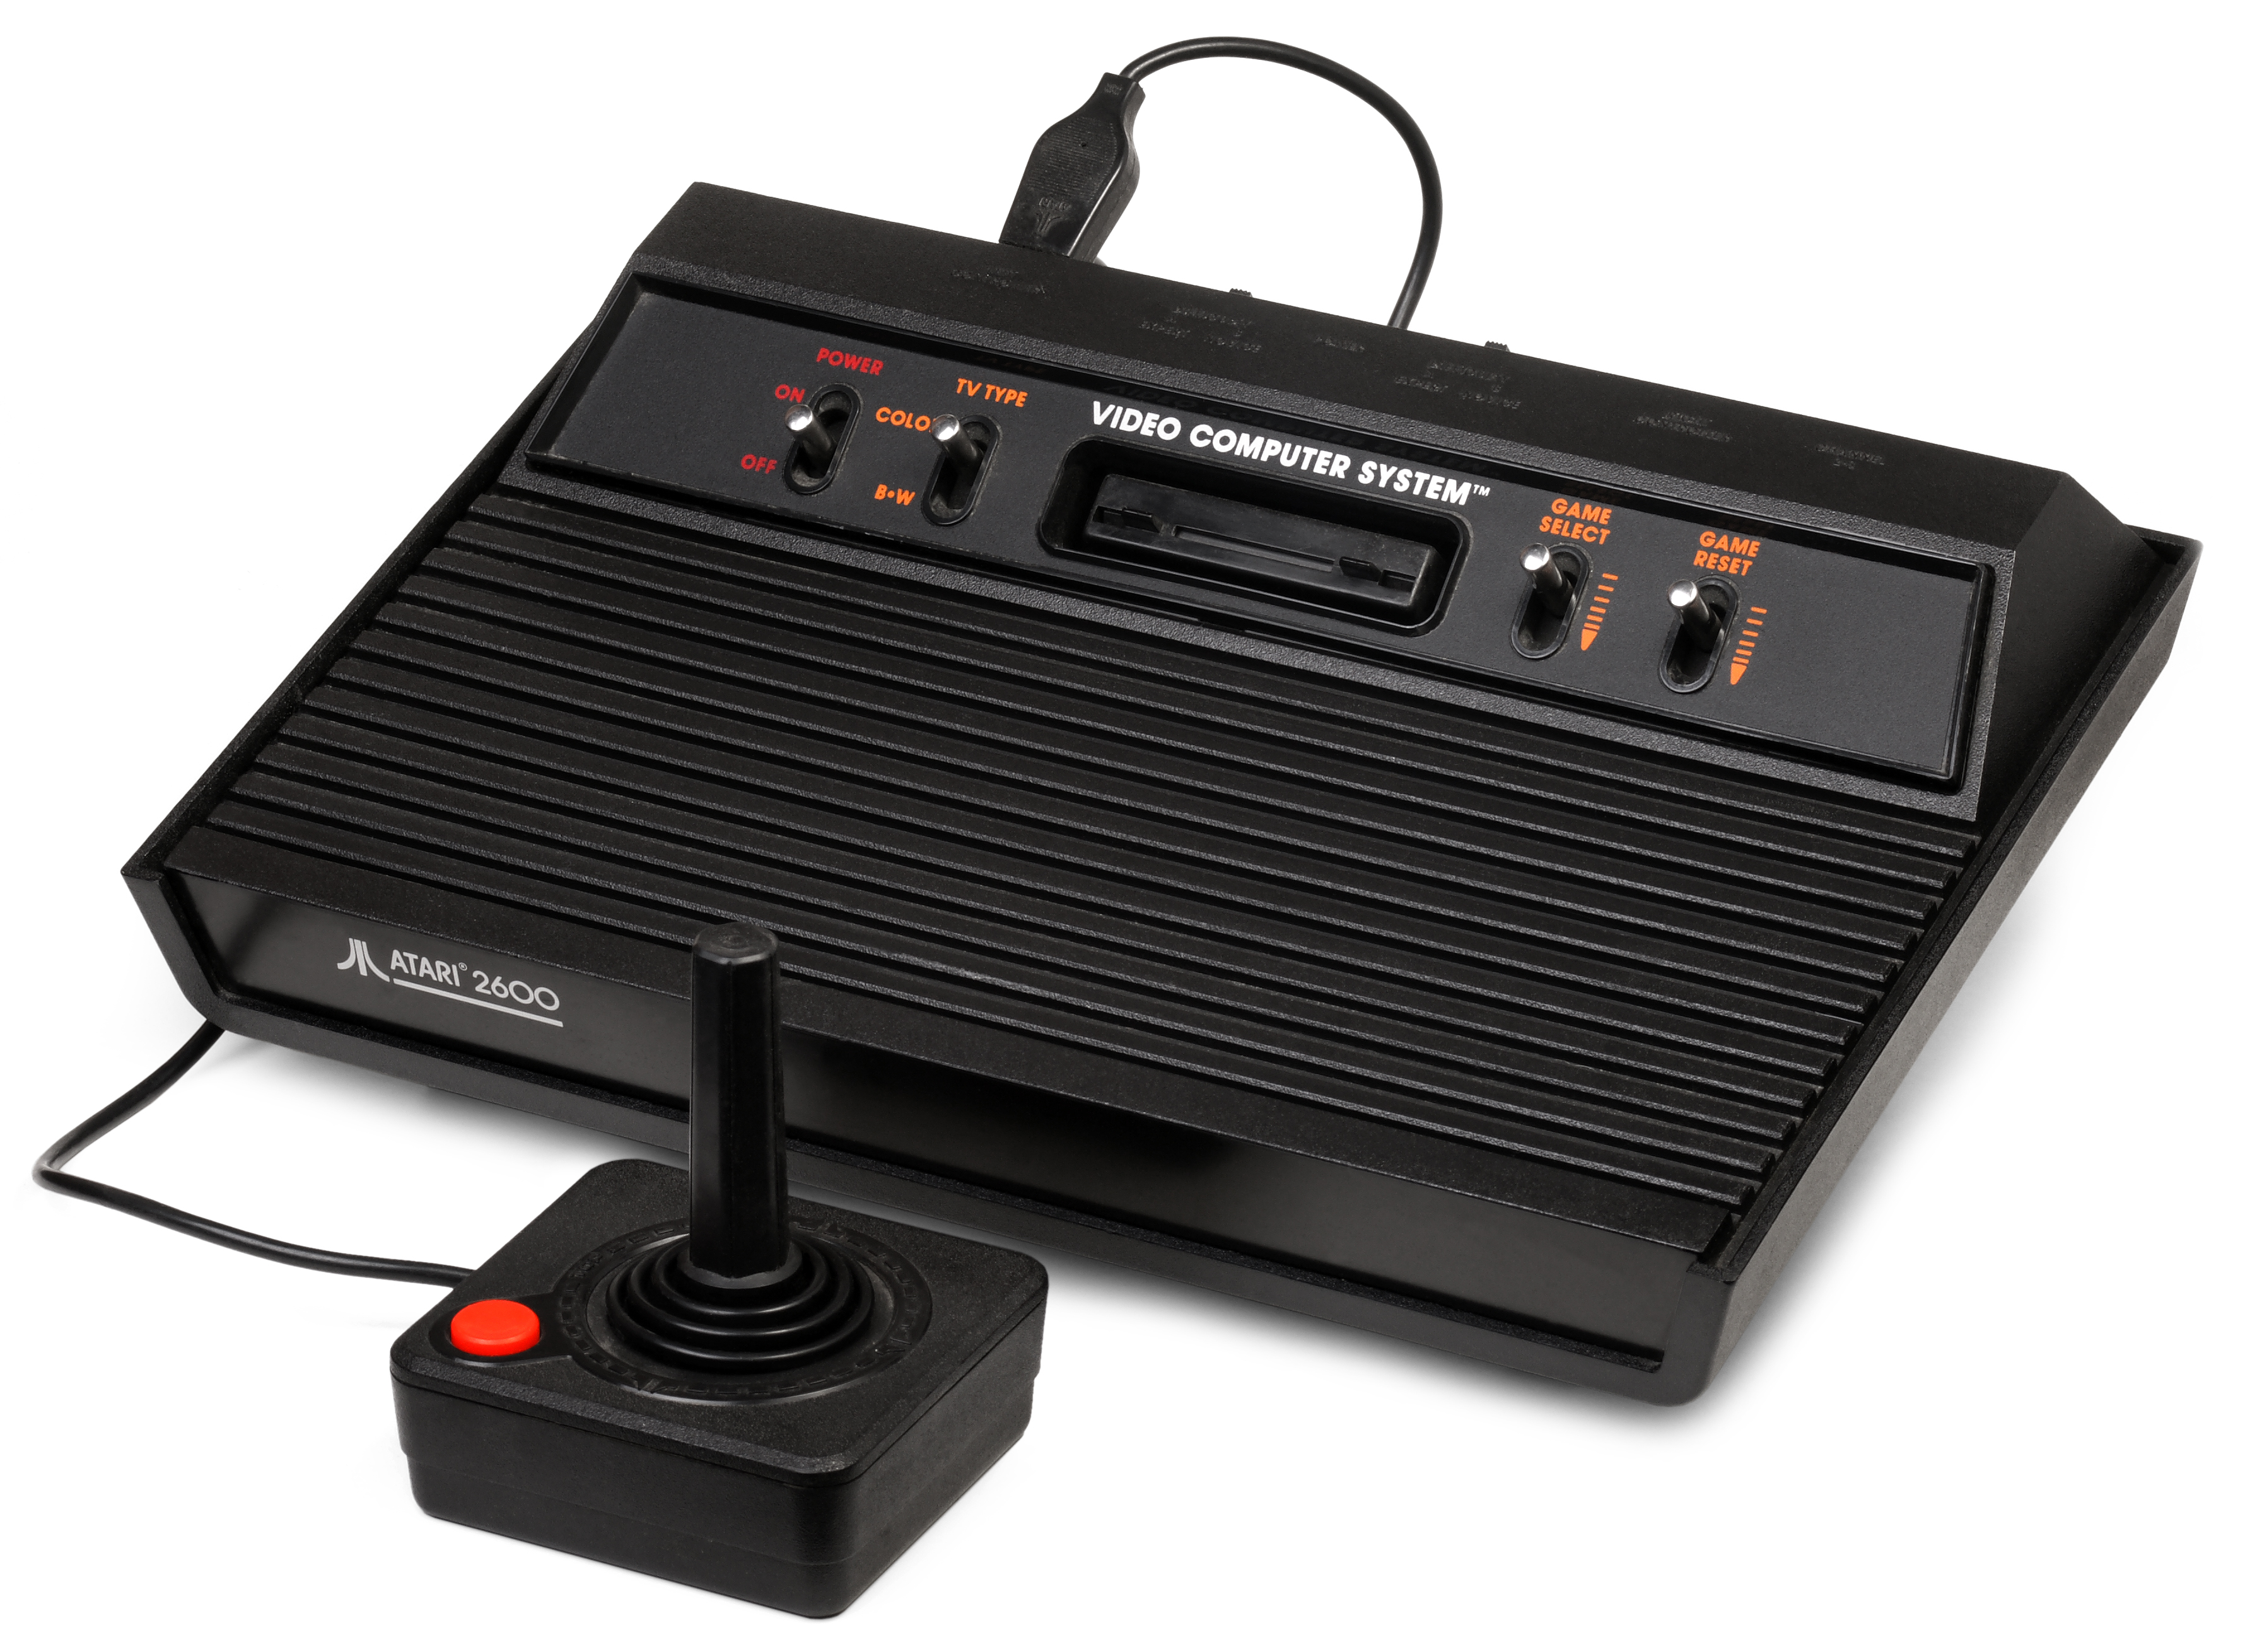
\includegraphics[width=90mm]{Atari2600Console.jpg}
	\caption{Hệ máy chơi game Atari 2600}
	\label{fig:AtariConsole}
\end{figure}

\section{Giới thiệu cấu trúc mạng và các siêu tham số đã chọn}
\section{Kết quả thực nghiệm}